\chapter{GAMBARAN UMUM}
Kabupaten Belitung Timur merupakan kabupaten yang terbentuk melalui Undang-Undang No. 5 Tahun 2003. Berdasarkan undang-undang tersebut Kabupaten Belitung Timur telah menjadi daerah otonom dalam Negara Kesatuan Republik Indonesia. Kabupaten Belitung Timur merupakan hasil pemekaran Kabupaten Belitung yang merupakan bagian dari Provinsi Bangka Belitung. Ibukota Kabupaten Belitung Timur adalah Kota Manggar yang berjarak sekitar 70 Km dari Kota Tanjungpandan yang merupakan Ibukota Kabupaten Belitung.

Kabupaten Belitung Timur secara \emph{de jure} \& \emph{de facto} terbentuk pada tanggal 24
Mei 2003 dengan ditetapkannya UU Nomor 5 Tahun 2003 serta dilantiknya
Pejabat Bupati Belitung Timur. Sejak tanggal 24 Mei 2003 tersebut
secara administratif Belitung Timur telah menjalankan roda pemerintahan
dengan mengacu kepada ketentuan hukum yang berlaku, dengan segala
kewenangan dan ketentuan yang menyangkut administrasi pemerintahan
dan kebijakan publik telah dilaksanakan dengan tetap berkoordinasi
kepada Pemerintah Pusat, Pemerintah Provinsi dan Pemerintah Kabupaten
Belitung.

\section{KEADAAN WILAYAH}

\subsection{Posisi Geografis}

Secara geografis Kabupaten Belitung Timur awalnya terdiri atas 4 kecamatan,
yang kemudian dimekarkan menjadi 7 kecamatan, berdasarkan Peraturan
Daerah Kabupaten Belitung Timur Nomor 3 Tahun 2011 Tentang Pembentukan
Kecamatan Damar, Kecamatan Simpang Renggiang, Kecamatan Dendang, dan
Kecamatan Simpang Pesak.

Kabupaten Belitung Timur memiliki luas wilayah 2.506,91 km², letak
geografis terletak antara 107°45' BT - 108°18' BT dan 02°30′ LS -
03°15′ LS. Batas-batas administrasi Kabupaten Belitung Timur adalah:
\begin{itemize}
	\item Utara : Selat Karimata
	\item Selatan : Laut Jawa
	\item Barat : Kabupaten Belitung
	\item Timur : Selat Karimata
\end{itemize}

Secara geografis Kabupaten Belitung Timur yang berada di koridor Selat
Karimata, merupakan salah satu potensi tersendiri yang dimiliki kawasan
ini.

\subsection{Batas Administrasi}

Kabupaten Belitung Timur terbagi dalam 7 (Tujuh) Kecamatan yakni
Kecamatan Manggar, Kecamatan Gantung, Kecamatan Kelapa Kampit, Kecamatan
Dendang, Kecamatan Simpang Pesak, Kecamatan Damar, dan Kecamatan Simpang
Renggiang. Dari 7 kecamatan tersebut batas administrasi dibagi lagi menjadi 39 (Tiga Puluh Sembilan) desa (\autoref{tab:Daftar-Kecamatan-Luas}).

\newpage

\begin{longtable}[H]{rlrl}
\caption{Daftar Kecamatan, Luas Wilayah, Jumlah Penduduk dan Nama Desa di Kab. Belitung Timur Tahun \tP}
\label{tab:Daftar-Kecamatan-Luas}
\\\toprule %longtable need to start with an explicit linebreak (\\)
No & Kecamatan & \makecell[r]{Luas\\Wilayah (km\textsuperscript{2})} & Desa\\
\midrule
\midrule
                 1 & Manggar           & 229     & Kelubi                 \\
                   &                   &         & Padang                 \\
                   &                   &         & Lalang                 \\
                   &                   &         & Lalang Jaya            \\
                   &                   &         & Kurnia Jaya            \\
                   &                   &         & Baru                   \\
                   &                   &         & Buku Limau             \\
                   &                   &         & Mekar Jaya             \\
                   &                   &         & Bentaian Jaya          \\ \midrule
                 2 & Damar             & 236,9   & Air Kelik              \\
                   &                   &         & Mempaya                \\
                   &                   &         & Burung Mandi           \\
                   &                   &         & Mengkubang             \\
                   &                   &         & Sukamandi              \\ \midrule
                 3 & Kelapa Kampit     & 498,5   & Cendil                 \\
                   &                   &         & Buding                 \\
                   &                   &         & Mentawak               \\
                   &                   &         & Senyubuk               \\
                   &                   &         & Mayang                 \\
                   &                   &         & Pembaharuan            \\ \midrule
                 4 & Gantung           & 546,3   & Gantung                \\
                   &                   &         & Jangkar Asam           \\
                   &                   &         & Batu Penyu             \\
                   &                   &         & Lenggang               \\
                   &                   &         & Lilangan               \\
                   &                   &         & Selinsing              \\
                   &                   &         & Limbongan              \\ \midrule
                 5 & Simpang Renggiang & 390,7   & Simpang Tiga           \\
                   &                   &         & Renggiang              \\
                   &                   &         & Aik Madu               \\
                   &                   &         & Lintang                \\ \midrule
                 6 & Simpang Pesak     & 362,2   & Simpang Pesak          \\
                   &                   &         & Tanjung Batu Itam      \\
                   &                   &         & Dukong                 \\
                   &                   &         & Tanjung Kelumpang      \\ \midrule
                 7 & Dendang           & 243,3   & Nyuruk                 \\
                   &                   &         & Balok                  \\
                   &                   &         & Jangkang               \\
                   &                   &         & Dendang                \\ \midrule
\multicolumn{2}{c}{Jumlah}             & 2.506,9 & \multicolumn{1}{c}{39}\\ %longtable need to ends with an explicit linebreak (\\)
\bottomrule
\end{longtable}

\section{KEADAAN PENDUDUK}
\subsection{Jumlah dan Kepadatan Penduduk}
Jumlah penduduk Kabupaten Belitung Timur pada tahun \tP diproyeksikan sebanyak
129.048 jiwa dengan kepadatan penduduk sebesar 51,48 orang/km\textsuperscript{2}.

\begin{figure}[H]
	\centering
	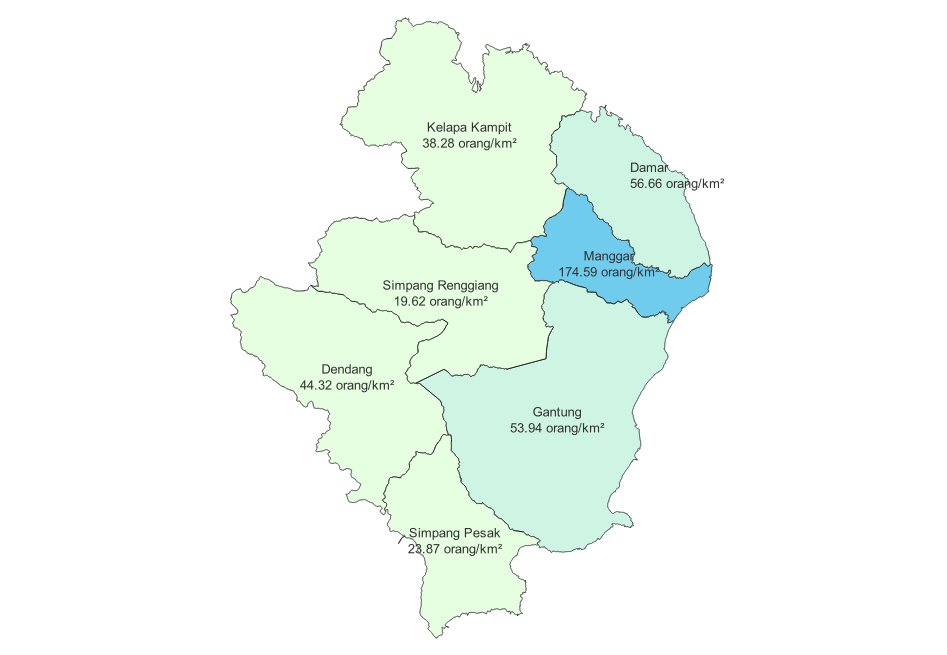
\includegraphics[width=0.85\textwidth]{bab_01/bab_01_01_kepadatanPenduduk}
	\caption{Kepadatan Penduduk di Kab. Belitung Timur Tahun \tP per Kecamatan}
	\label{fig:Kepadatan-Penduduk}
\end{figure}

Bila dikaitkan dengan pola distribusi secara spasial (\autoref{fig:Kepadatan-Penduduk}), maka terlihat
bahwa Kecamatan Manggar merupakan kecamatan dengan tingkat kepadatan
penduduk paling tinggi, sementara Kecamatan Simpang Renggiang merupakan
kecamatan dengan tingkat kepadatan penduduk paling rendah.

\subsection{Proporsi Penduduk Menurut Umur}
Proporsi penduduk menurut umur di Kabupaten Belitung Timur tahun
\tP dapat dilihat pada Piramida Penduduk Kab. Belitung Timur Tahun \tP (~\autoref{fig:Piramida-Penduduk-2022}).

\begin{figure}[!h]
    \centering{}
    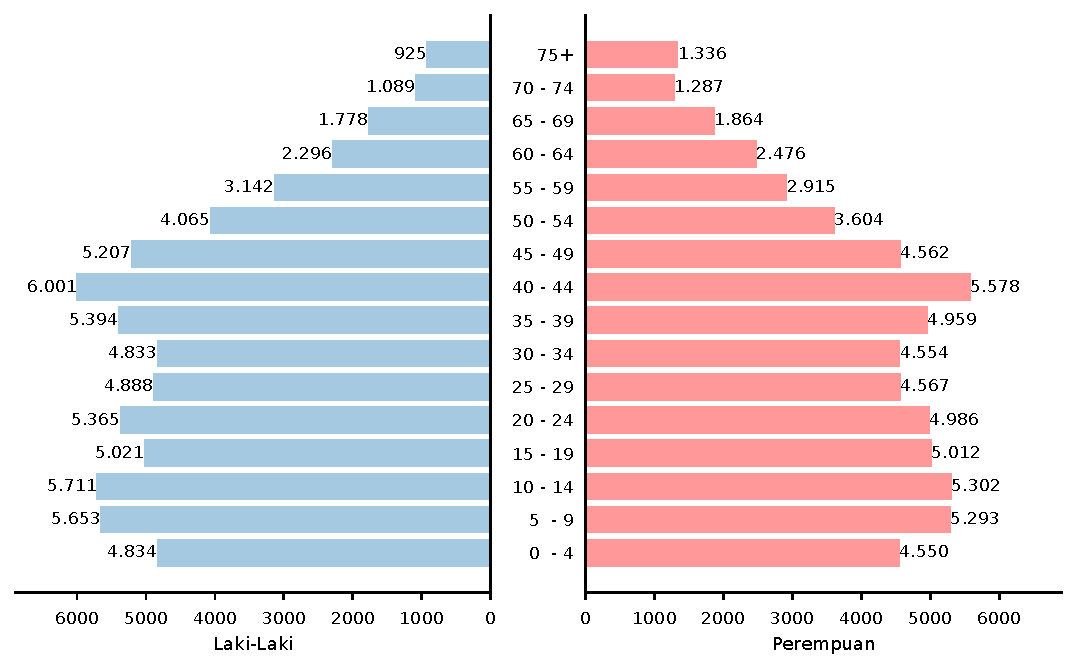
\includegraphics[width=\textwidth]{bab_01/bab_01_1_piramidaPenduduk}
%    \noindent\shadowimage[width=.9\textwidth]{bab_01/bab_01_1_piramidaPenduduk}
    \caption{Piramida Penduduk Kab. Belitung Timur Tahun \tP}
    \label{fig:Piramida-Penduduk-2022}
\end{figure}

Rasio beban tanggungan di kabupaten Belitung Timur adalah 44,31, yaitu setiap 100 orang penduduk usia produktif (umur 15 – 64 tahun) menanggung 44,31 orang penduduk usia non produktif (umur 0 – 14 tahun dan 65 – 75+ tahun).

\subsection{Proporsi Penduduk Menurut Jenis Kelamin}
Kabupaten Belitung Timur pada tahun \tP diproyeksi memiliki jumlah penduduk laki-laki sebesar 66.201 orang dan jumlah penduduk perempuan sebesar 62.847 orang, dengan total keseluruhan jumlah penduduk Kabupaten Belitung Timur yaitu 129.048 jiwa. Dengan demikian proporsi penduduk laki-laki adalah 51,30\% sedangkan proporsi penduduk perempuan adalah 48,70\% dengan rasio jenis kelamin sebesar 105,34 (\autoref{fig:Proporsi-Penduduk-Gender}).

\begin{figure}[!h]
    \centering{}
%    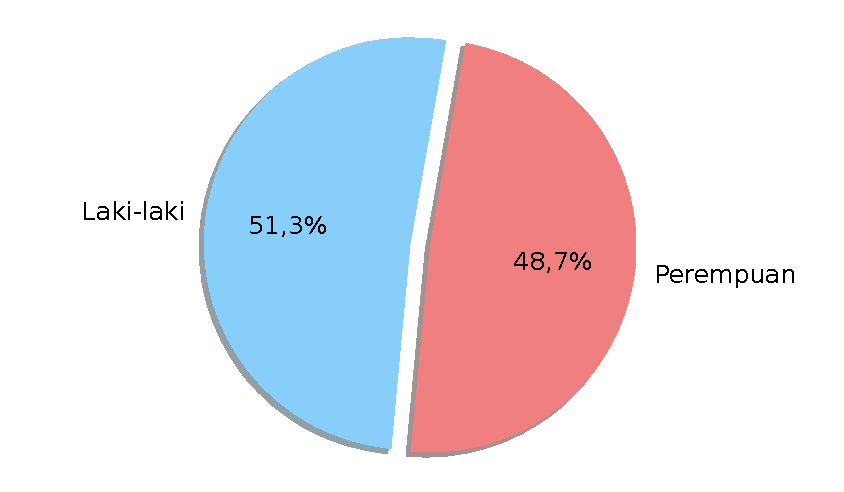
\includegraphics[width=0.7\textwidth]{bab_01/bab_01_2_distribusiGender}
%%    \noindent\shadowimage[width=.7\textwidth]{bab_01/bab_01_2_distribusiGender}
    \caption{Proporsi Penduduk Kab. Belitung Timur  Tahun \tP Menurut Jenis Kelamin}
    \label{fig:Proporsi-Penduduk-Gender}
\end{figure}

\section{KEADAAN PENDIDIKAN}
Komponen pengukuran tingkat pembangunan manusia suatu negara yang
cukup berpengaruh yaitu komponen pendidikan. Perubahan yang terjadi
secara terus menerus pada perilaku masyarakat disebabkan oleh semakin
meningkatnya tingkat pendidikan. Pendidikan juga merupakan salah satu
syarat mutlak pencapaian tujuan pembangunan manusia, dan merupakan
target pembangunan sekaligus sarana pembangunan nasional.

Salah satu capaian dalam bidang pendidikan yaitu kepemilikan ijazah
atau Surat Tanda Tamat Belajar (STTB), yang pada akhirnya akan menjadi
jalan untuk melanjutkan pendidikan ke jenjang pendidikan yang lebih
tinggi atau menjadi dasar untuk mencari pekerjaan yang sesuai. Selain
itu, ijazah/ STTB biasanya juga menjadi tolok ukur dalam pergaulan
atau hubungan sosial. Terkait dengan kualitas hidup manusia, ada kecenderungan semakin tinggi
ijazah/ STTB yang dimiliki maka pengetahuan pun semakin banyak dan
berakibat pada meningkatnya kualitas hidup terutama di bidang kesehatan
dan perumahan.

Pada tahun \tP diperkirakan terdapat 10,49\% penduduk Kabupaten Belitung Timur berusia di atas 15 tahun yang tidak memiliki ijazah SD/ sederajat. Sebanyak 32,26\% penduduk memiliki ijazah tertinggi berupa pendidikan dasar, yaitu telah menamatkan pendidikan SMA atau sederajat. Sebanyak 7,74\% penduduk telah menamatkan pendidikan tinggi (Diploma/ Sarjana) (\autoref{fig:Tingkat-Pendidikan}).

\begin{figure}[H]
    \centering
%    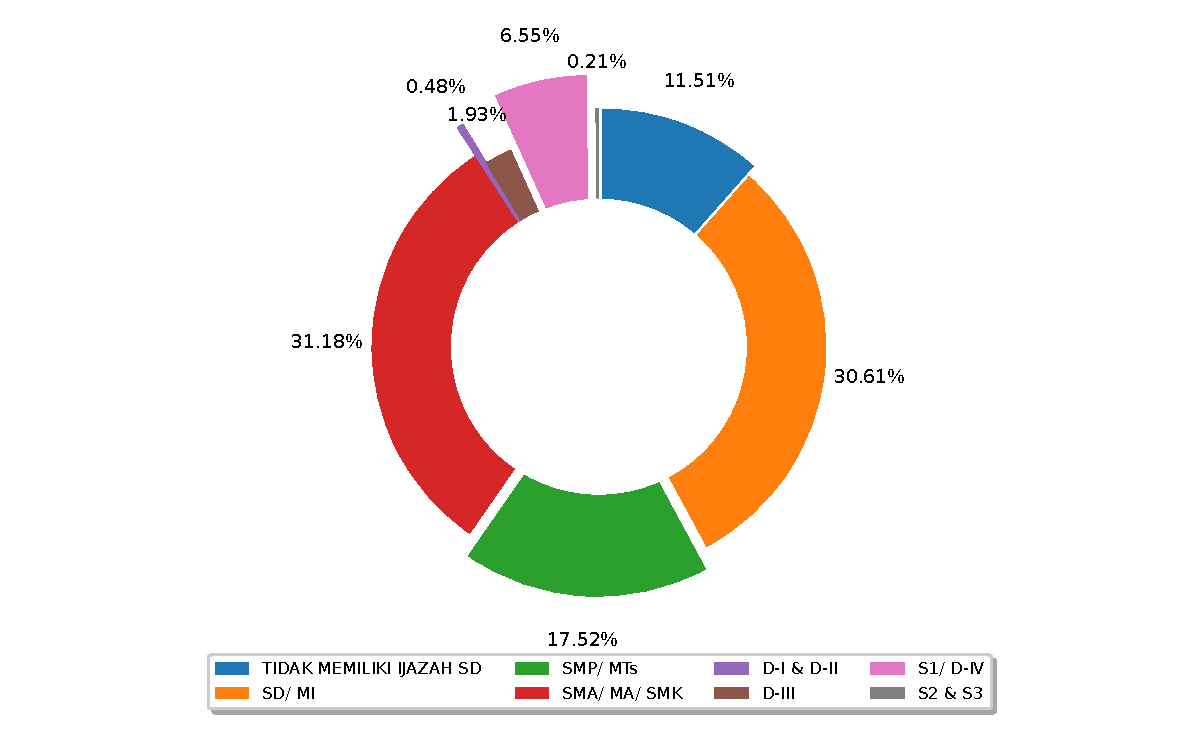
\includegraphics[width=0.9\textwidth]{bab_01/bab_01_03_distribusiPendidikan}
%    %\shadowimage[width=.7\textwidth]{bab_01/bab_01_03_distribusiPendidikan}
    \caption{Distribusi Penduduk Kab. Belitung Timur Tahun \tP Menurut Tingkat Pendidikan}
    \label{fig:Tingkat-Pendidikan}
\end{figure}
